% !TEX root = main.tex

\chapter{Instabilities of a potential free-surface vortex flow}

\begin{description}
\item{Directory in the StabFem project :}  \texttt{ROTATINGPOLYGONS}
\item{Main contributors :} J. Mougel, D. Fabre
\item{Reference :} Mougel et al., JFM 2018 
\end{description}

\begin{figure}
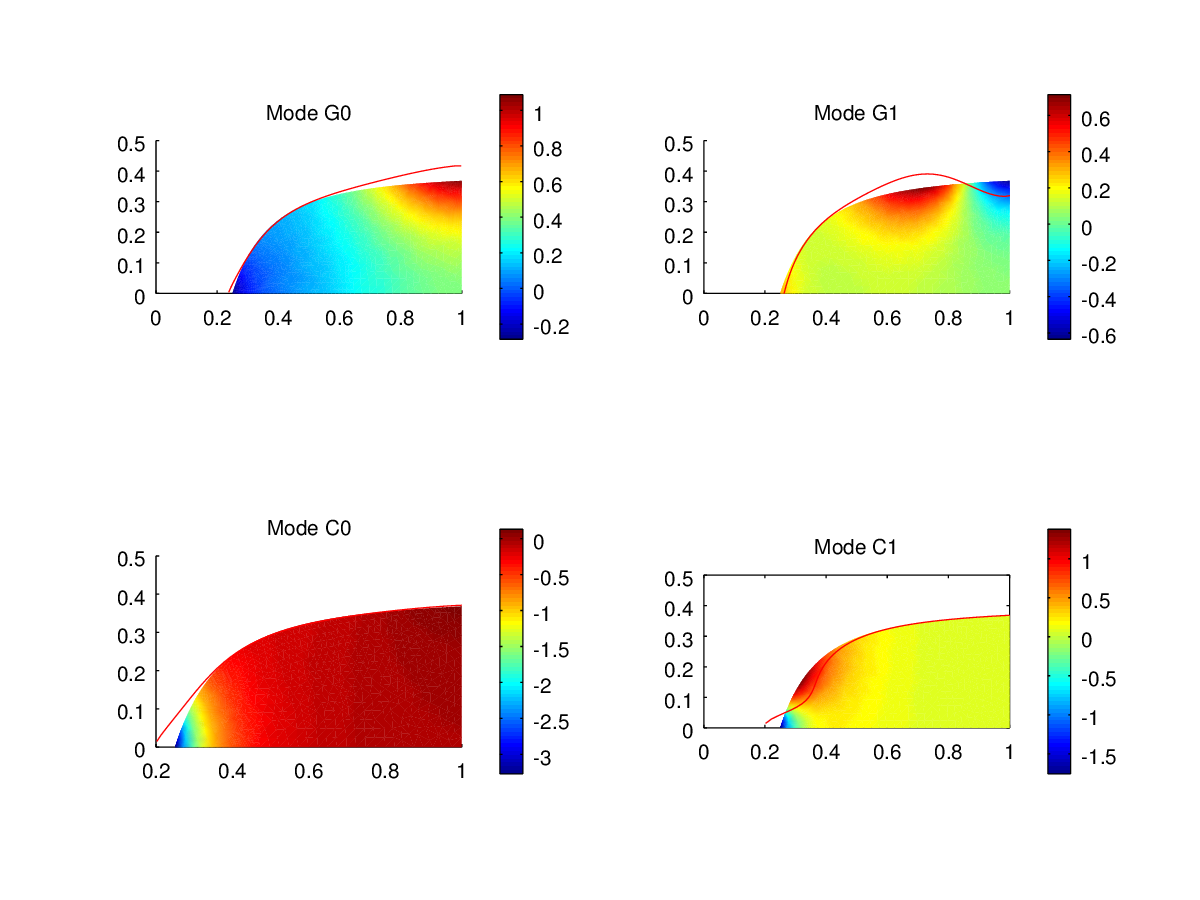
\includegraphics[width=.8\linewidth]{../ROTATING_POLYGONS/FIGURES/POLYGONS_modes.png}
\caption{Oscillation modes of a potential vortex for  $a=H/R=0.3$ and $m=3$ (figure 5, 6 of Mougel et al.).}
\label{Bridges_NV_Eigenmodes_phi_cyl_L3_5}
\end{figure}

\begin{figure}
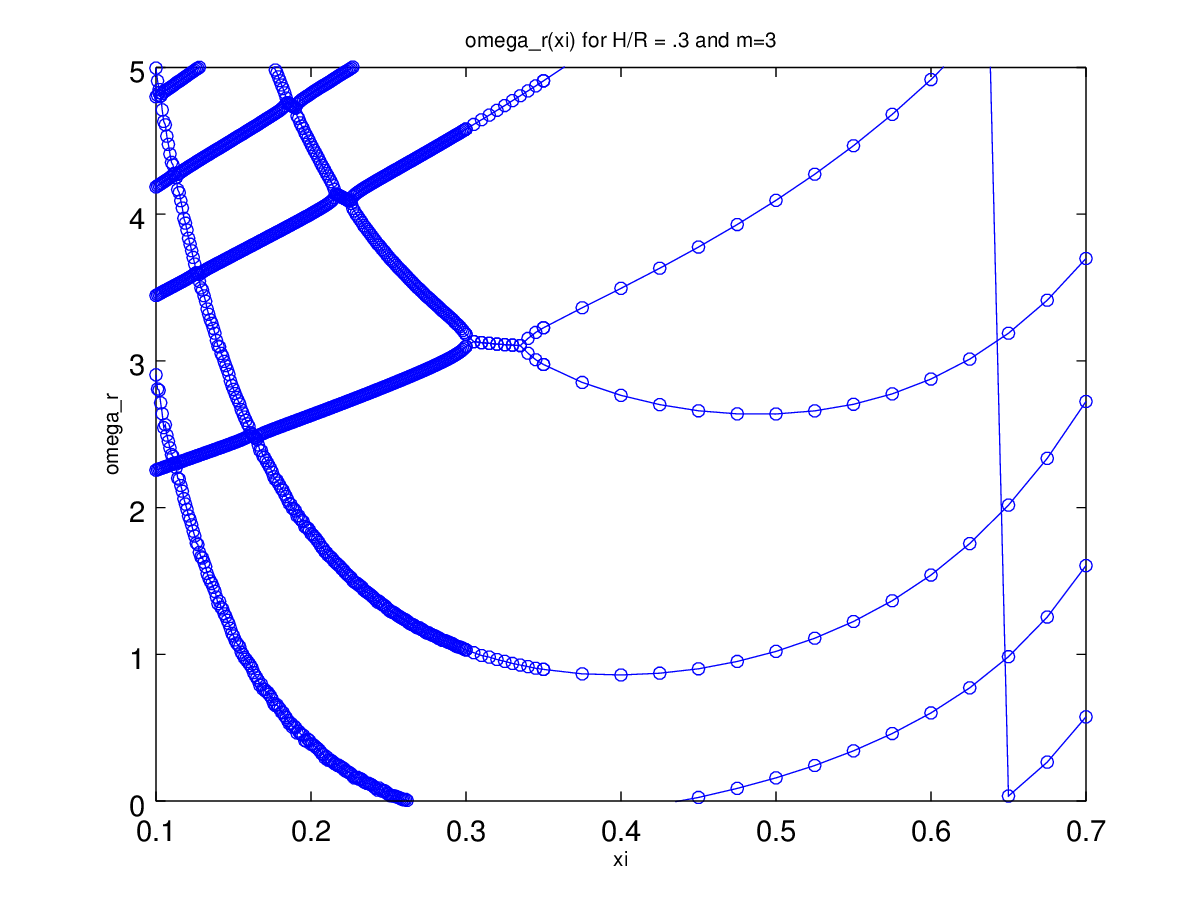
\includegraphics[width=.45\linewidth]{../ROTATING_POLYGONS/FIGURES/POLYGONS_omega.png}
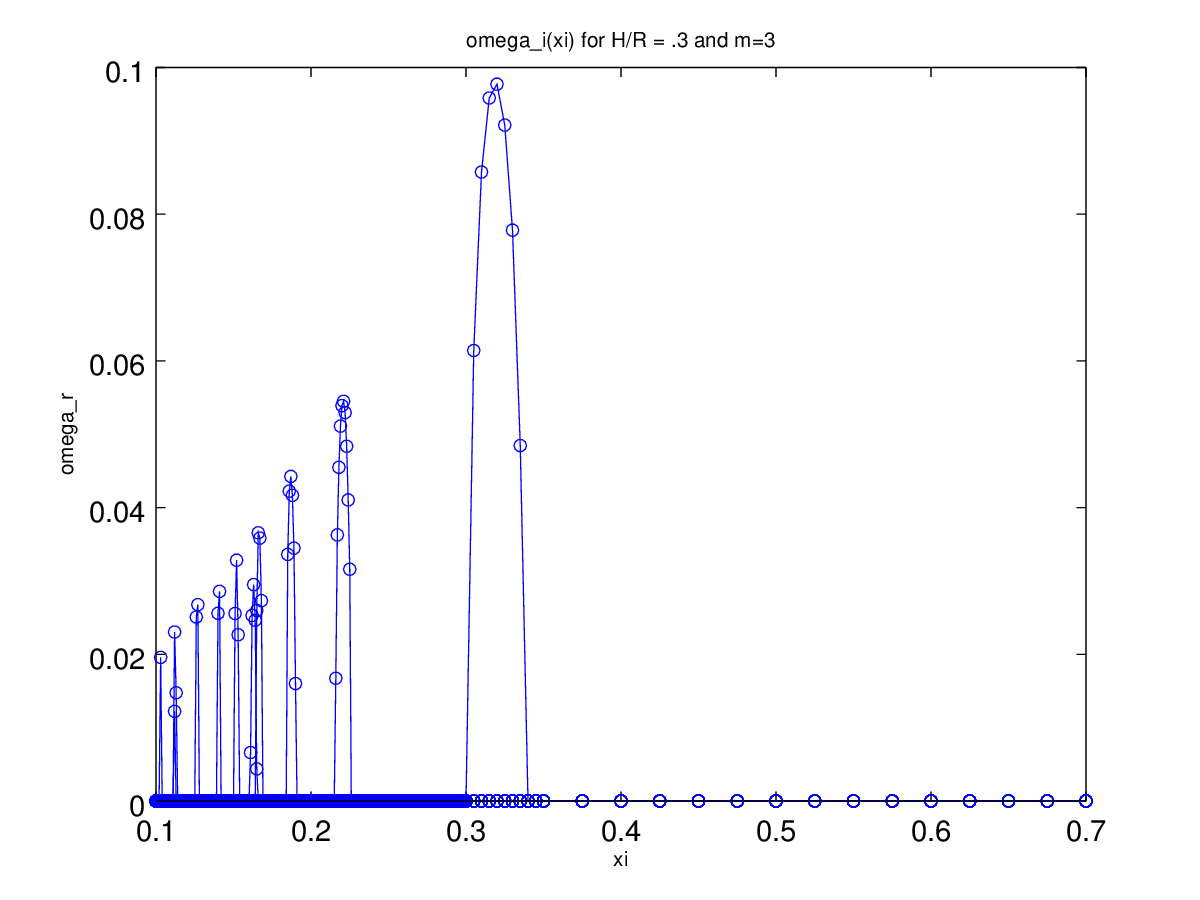
\includegraphics[width=.45\linewidth]{../ROTATING_POLYGONS/FIGURES/POLYGONS_sigma.png}
\caption{Oscillation frequencies and amplification rates for f a potential vortex for $m=3$ (figure 4 of Mougel et al.).}
\label{Bridges_NV_Eigenmodes_phi_cyl_L3_5}
\end{figure}
 